\section{Result and Discussion}
In the present study, the T300/5308 graphite/epoxy material is used in the
lay-up sequence optimization, and its properties as shown in
table.\ref{tab:T300/5308}. Two constraints are imposed on the composite
laminates which are the safety factor $SF_{MS}$ , and safety factor $SF_{TW}$,
and the threshold values for both of them is 1. The constraint values of an
individual are $CV_1$ and $CV_2$. So the mutation vector here is a two-dimensional
vector $[1 - CV_1, 1 - CV_2 ]$, and the coefficient of length
mutation $C_l$ and angle mutation $C_a$ are  20 and 10, respectively.

To verify the reliability of the proposed method, two conditions are concerned: the
first is only two distinct fiber orientation angles in the composite material;
the second involves three distinct ply angles within the optimization process.
In each situation, first, we present the search process by plotting relevant
indicators, such as the fitness, strength ratio, and angle. Then, the optimum
lay-ups under various loading cases are discussed.

\begin{figure}[!htb]
	\centering
		\begin{subfigure}[b]{0.8\linewidth}
			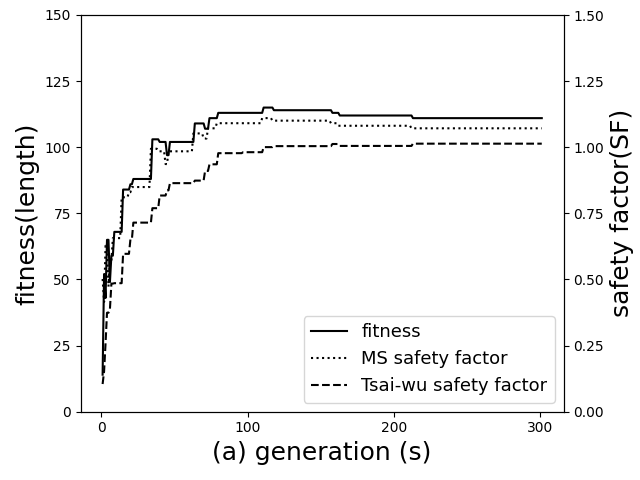
\includegraphics[width=\linewidth]{2020-11-10-pre-image/two_distinct_angle_fitness_and_sr.png}
		\end{subfigure}

		\begin{subfigure}[b]{0.8\linewidth}
			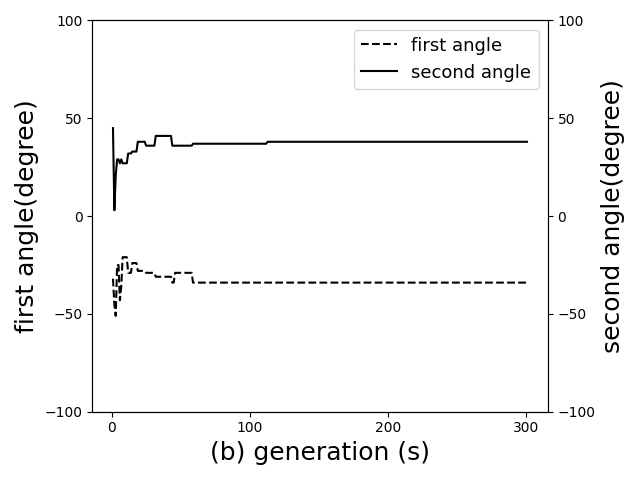
\includegraphics[width=\linewidth]{2020-11-10-pre-image/two_distinct_angle_angle_change.png}
		\end{subfigure}

		\begin{subfigure}[b]{0.8\linewidth}
			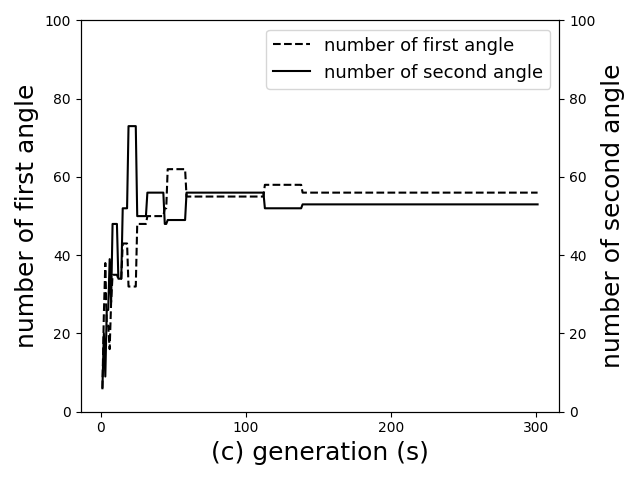
\includegraphics[width=\linewidth]{2020-11-10-pre-image/two_distinct_angler_number_change.png}
		\end{subfigure}
	\caption{Two distinct angles}
	\label{fig:two_angles}
\end{figure}


\begin{table*}
	\normalsize
\caption{The optimum lay-ups using two distinct fiber angles under various biaxial loading cases}
\label{tab:two_distinct_angle}
\centering
\begin{tabular}{clccc}
	\toprule
	\textbf{Loading} $N_{x}/N_{y}/N_{xy}$ \textbf{(MPa m)}   &
	\makecell{\textbf{Optimum lay-up } \\ \textbf{sequences}  }                        &
	\textbf{Laminate thickness} &  \makecell{\textbf{Safety factor } \\
	\textbf{for Tsai-wu}}  &
	\makecell{\textbf{Safety factor } \\ \textbf{for  maximum stress}}
	 \\
	\midrule
	10/5/0                                         &  $[33_{29}/\text{-}39_{25}/\bar{\text{-}39}]_s$            &     109               &  1.0074      &  1.0246  \\
	20/5/0                                         &  $[33_{22}/\text{-}31_{24}]_s$                             &     92               &  1.0055       &  1.2065    \\
	40/5/0                                         &  $[29_{18}/\text{-}21_{23}/\bar{\text{-}21}]_s$            &     83               &  1.0034       &  1.7350   \\
	80/5/0                                         &  $[\text{-}20_{27}/21_{25}/\bar{25}]_s$                    &     105               &  1.0029      &  1.2063    \\
	120/5/0                                         &  $[\text{-}18_{34}/17_{36}]_s$                            &     140               &  1.0000      &  1.0898    \\
	\bottomrule
\end{tabular}
\end{table*}

Figure \ref{fig:two_angles}(a) shows how the optimal individual's fitness and
strength ratio evolves during the GA process. The solid curve shows the fitness
value, the dashed curve shows the Tsai-wu safety factor, and the dotted curve
shows MS safety factor. If the smaller strength ratio fullfills the constraint,
this laminate must satisfy all the constraints, for simplicity, only the smaller
strength ratio is presented in the figure\ref{fig:three_angles}(a). The method
to chose optimal individual considering two following situations, if no
individual in the current population meets constraint, the one with the biggest
fitness is selected as the optimal individual; if there are one or multiple
individuals fullfills requirement, the one with the smallest fitness is chosen which
means the smallest one has the biggest priority.  Figure \ref{fig:two_angles}
(b) and \ref{fig:three_angles}(b) show how every fiber orientation changes, and
Figure \ref{fig:two_angles}(c) and \ref{fig:three_angles}(c) display how the
number of each angle varies.

At the beginning of this GA process, the fitness curves increases very quickly,
because individual's two strength ratios are very small, so the difference
between the individual's fitness and the imposed constraint threshold is a big
positive number, so the range of mutation length is from 0 to $C_l(CT_0 - CV_0 +
CT_1 - CV_1)/2$.  The length of individual increases by n, which is a random
number between 0 and $C_l(CT_0 - CV_0 + CT_1 - CV_1)/2$ . As can be seen from
Figure \ref{fig:two_angles} (a), both of optimal individual's fitness and
strength ratio increases very quickly.  The range of angle mutation is from 0 to
$C_a(CT_0 - CV_0 + CT_1 - CV_1)/2$, and the number of each angle also changes
violently. The Figure.\ref{fig:two_angles} (a) and \ref{fig:three_angles} (a) show
this property at the initial stage.  During this stage, increasing an individual's length playing a
major role in increasing its fitness.

After a couple of generations, the optimal individual's fitness gets bigger, and
the difference between individual's fitness and constraint threshold gets
smaller. The range of mutation length turns smaller. At
this stage, simply increase the individual's length doesn't make much difference
in improve an individual's fitnees, and a better composite laminates lay-up can
dramatically change the optimal individual's fitness. That's why the fitness curve
oscillated violently in this stage.  At the same time, the strength ratio curve
keeps growing smoothly. But the growing speed gets more smaller.

When GA comes to its last phase, GA finds individuals that meet all the
constraints.  Now the optimal individual's fitness is greater than the safety
factor. The range of mutation length is from $C_l(CT_0 - CV_0 + CT_1 - CV_1)/2$
to 0. It means individuals need to decrease its length and improve its internal
structure to meet the constraint. That's why the fitness of optimal individual
kept decreaing, however, the strength ratio curve still is greater than safety
factor.

\begin{figure}[!t]
	\centering
		\begin{subfigure}[b]{0.8\linewidth}
			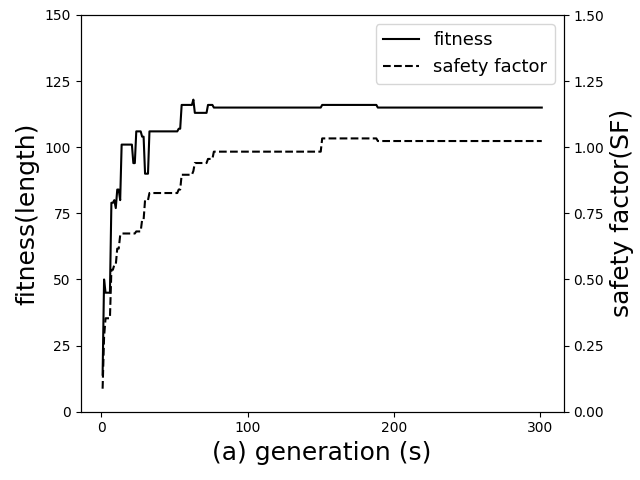
\includegraphics[width=\linewidth]{2020-11-10-pre-image/Three_distinct_angles_fitness_and_sr.png}
		\end{subfigure}

		\begin{subfigure}[b]{0.8\linewidth}
			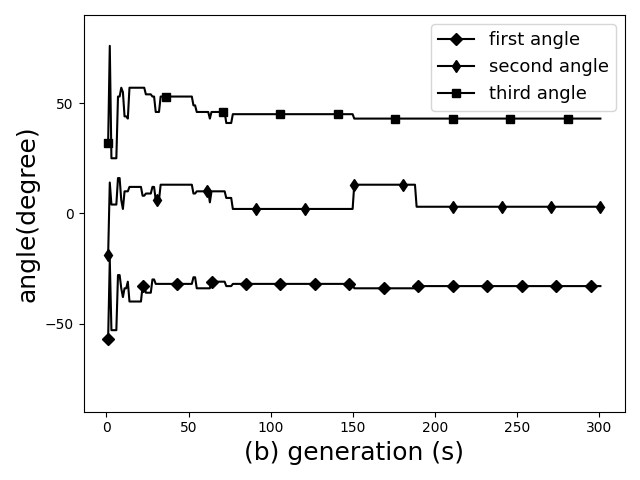
\includegraphics[width=\linewidth]{2020-11-10-pre-image/three_distinct_angles_angle_change.png}
		\end{subfigure}

		\begin{subfigure}[b]{0.8\linewidth}
			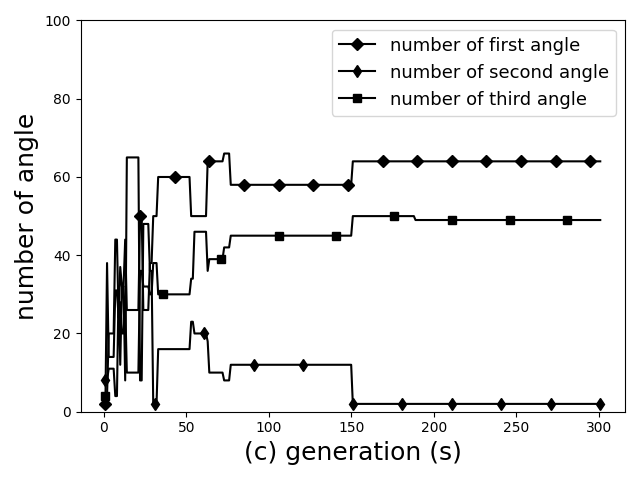
\includegraphics[width=\linewidth]{2020-11-10-pre-image/three_distinct_angle_number_of_angle.png}
		\end{subfigure}
	\caption{Three distinct angles}
	\label{fig:three_angles}
\end{figure}


\begin{table*}
\normalsize
\caption{The optimum lay-ups using three distinct fiber angles under various biaxial loading cases}
\label{T300/5308 material properties}
\centering
\begin{tabular}{clccc}
	\toprule
	\textbf{Loading} $N_{x}/N_{y}/N_{xy}$ \textbf{(MPa m)}   &
	\makecell{\textbf{Optimum lay-up } \\ \textbf{sequences}  }                        &
	\textbf{Laminate thickness} &  \makecell{\textbf{Safety factor } \\
	\textbf{for Tsai-wu}}  &
	\makecell{\textbf{Safety factor } \\ \textbf{for  maximum stress}}
	 \\
	\midrule
	10/5/0                       &  $[37_{27}/\text{-}38_{27}/\text{-}5]_s$            &     110      &  1.0023 & 1.0216\\
	20/5/0                       &  $[34_{24}/\text{-}32_{14}/\text{-}28_{11}]_s$      &     98       &  1.0237 & 1.2089 \\
	40/5/0                       &  $[21_{28}/\text{-}32_{19}/2_3]_s$                  &     100      &  1.0617 & 1.7076\\
	80/5/0                       &  $[\text{-}19_{24}/20_{27}/\text{-}{17}_{16}/\bar{\text{-}17}]_s$  &  109      &  1.0056 & 1.2093 \\
	120/5/0                      &  $[\text{-}19_{33}/12_{13}/16_{28}]_s$              &     148      &  1.0105 &  1.1014\\
	\bottomrule
\end{tabular}
\end{table*}

\begin{table*}
	\normalsize
\caption{Comparison with the results of DSA}
\label{tab:comparision}
\centering
\begin{tabular}{c|cccc|lccc}
	\toprule
	\textbf{Loading}	    & \multicolumn {4}{c}{\textbf{Akbulut and Sonmez's\cite{akbulut2008optimum} Study}}   & \multicolumn {4}{c}{\textbf{Present Study}}\\
	\midrule
	 $N_{x}/N_{y}/N_{xy}$   & Optimum lay-up			        & laminate  & TW & MS   & Optimum lay-up & laminate  & TW & MS \\
	  (MPa m)	            & sequences					        & thickness &    &      & sequences	     & thickness &    &    \\
	\midrule
	  10/5/0                 &  $[37_{27}/\text{-}37_{27}]_s$     &  108      &  1.0068  &  1.0277 & $[33_{29}/\text{-}39_{25}/\bar{\text{-}39}]_s$     &     109      &  1.0074      &  1.0246  \\
	  20/5/0                 &  $[31_{23}/\text{-}31_{23}]_s$     &  92       &  1.0208  &  1.1985 & $[33_{22}/\text{-}31_{24}]_s$                      &     92      &  1.0055       &  1.2065    \\
	  40/5/0                 &  $[26_{20}/\text{-}26_{20}]_s$     &  80       &  1.0190  &  1.5381 & $[29_{18}/\text{-}21_{23}/\bar{\text{-}21}]_s$     &     83      &  1.0034       &  1.7350   \\
	  80/5/0                 &  $[21_{25}/\text{-}19_{28}]_s$     &  106      &  1.0113  &  1.2213 & $[\text{-}20_{27}/21_{25}/\bar{25}]_s$             &     105      &  1.0029      &  1.2063    \\
	  120/5/0                &  $[17_{35}/\text{-}17_{35}]_s$     &  140      &  1.0030  &  1.0950 & $[\text{-}18_{34}/17_{36}]_s$                     &     140      &  1.0000      &  1.0898     \\
	\bottomrule
\end{tabular}
\end{table*}

Table.\ref{tab:comparision} shows the comparison with the result obtained by
direct search simulated annealing(DSA) algorithm which was proposed by Akbulut
and Sonmez\cite{akbulut2008optimum}.  Both of variant GA and DSA are able to
find feasible solution, but when loading is $N_x=80$, $N_y=5$ MPa m, variant GA
got a better solution than DSA. In the case that loadings are $N_x=20$, $N_y=5$ MPa m,
and $N_x=120$, $N_y=5$ MPa m,  the proposed GA offered an alternative solution. Compared
with DSA method, the last advantage of variant GA is the number of layers
doesn't have to be even.

